\chapter{Introduction}
\label{sec:intro}

Transmission performance has been an ever-lasting pursuit of network engineers and researchers since the dawn of Internet. 
The pursuit is stemmed from the distributed routing behavior and the hop-by-hop resource allocation mechanism that ensure the prevalence of this collection of individually manged networks.
With in the realm of Internet, networks and hosts alike selfishly compete for resources on common parts of paths, giving rise to congestion and sub-optimal global traffic distribution.

One major roadblock to better performance is insufficient network capacity. It is thus necessary to regularly perform network dimensioning and deployment, to ensure that the network capacity grows in line with traffic demands~\cite{pioro2004routing}. 
Among all sections in Internet, access network has a notorious reputation as performance bottleneck for a long time. 
Over last few years, new generations of access methods~\cite{Kramer2002, kazovsky2007next} have been greatly expanding the pipe of this `last mile'. 

Yet, congestion might still take place due to sudden increase of traffic demand for instance. End-to-end congestion control mechanism plays an important role here to optimize the performance in an distributed fashion.  
It aims at fully utilizing bottleneck bandwidth while introducing minimum additional transmission delay (short queue length) and ensuring fair share of resources~\cite{Jacobson1988, mathis1997macroscopic, Cardwell2016}.
%Recently emerging QUIC~\cite{roskind2012quick} and HTTP/2~\cite{belshe2015hypertext} further alleviate unfair resource share caused by multiple simultaneous connection through multiplexing.

However, the routing of Internet traffic might fail to take full advantage of available capacity, due to performance agnostic routing schemes, lack of global visibility, etc.
A cure to this sub-optimal traffic distribution is to exploit the diverse Internet paths potentially available.
Certain applications, e.g. skype and bitTorrent, built an application level connectivity overlay on top of the Internet topology that reveals richer end-to-end path diversity and leads to better resilience and performance.
MPTCP~\cite{Han2006} and QUIC~\cite{roskind2012quick} take advantage of the multiple available network connections, e.g. WiFi and mobile data, on an end host.
On a larger scale, each network when connecting to the rest of the Internet through multiple providers, is exposed to multiple available paths to reach destinations. Wisely choose these routes can thus as well yield considerable performance gain.

%\paragraph*{Internet path and traffic pattern shift}
%The rise of \acf{CDN} and large \ac{CP} such as Google and Facebook drastically reduces the physical distance between contents and eyeballs, hence decreases the overall transmission latency.
%The rapid growth of \acf{IXP} flattens the previous hierarchical Internet topology, and thus as well shortens Internet paths~\cite{Labovitz2011}.

The above mentioned approaches complement each other in achieving better transmission performance across Internet.
Yet, how to take advantage of path diversity at network level witnessed much less progress as other directions do.
Back to the beginning of this century, researchers already realized that multihoming and hence produced network level path diversity had the potential for performance boost.
Commercial products claiming capable of intelligent routing once emerged.
Then, they disappeared.
These systems were at best load balancers over transit links, thus could not fully address the end-to-end performance issue on a per destination base.

One major obstacle in this pursuit is that the routing protocol among different networks, i.e.\acf{BGP}, is unaware of performance differences across available paths.
One still available commercial product~\cite{b6} conducts regular performance measurements that are further considered in dynamic route selection, e.g. comparing measurements to a delay or increase amplitude threshold.
The academic world responded as well to the challenge, with more sophisticated route selection algorithms relying on historical measurements. 

A recent big news in the domain is that Google revealed \textit{Espresso}~\cite{espresso}. It is a \ac{SDN} component that dynamically selects Internet routes based on the instrumentation tailored for Google applications.
However, path diversity is no longer the privilege of large networks that can afford the technical and financial cost of such customized systems.
As transit price drops, multihoming becomes rather a common practice of numerous medium and small size networks. 
These networks as well have the immediate need for performance optimization so that their business could survive.

Despite the concrete need that is becoming more obvious day by day, many questions remain unanswered, or partially addressed.
A typical network can communicate with $\sim$ 100k different destinations regularly. 
Continuously measuring the performance to all that many destinations are costly and not necessary. 
What are the most important destinations to focus on? Do these destinations change over time? How to identify them?
Besides volume measurements, how should performance measurements be processed? Do they need cleaning?
If yes, what are the potential data quality issues? What are the origins of these issues? How can we showcase and mitigate their impacts on route selection?
Further, in order to dynamically react to performance changes, how to detect in first place significant changes in performance measurements? How to do so without hard-coded or ad hoc parameters, yet featuring an acceptable level of robustness?
Finally, once a performance change is detected, how can we learn more about this event from a network perspective? Where does it happen? Does it potentially impact other Internet paths currently in use? 
We aim to explore answers to above questions in this dissertation, so that the building of measurement-based route selection system advances in these aspects: measurement scalability, interpretation of performance data and visibility on causes of performance changes. 

\chapter{Background, scope and roadmap}
\section{Intradomain Routing}
\begin{figure}[!htb]
\centering
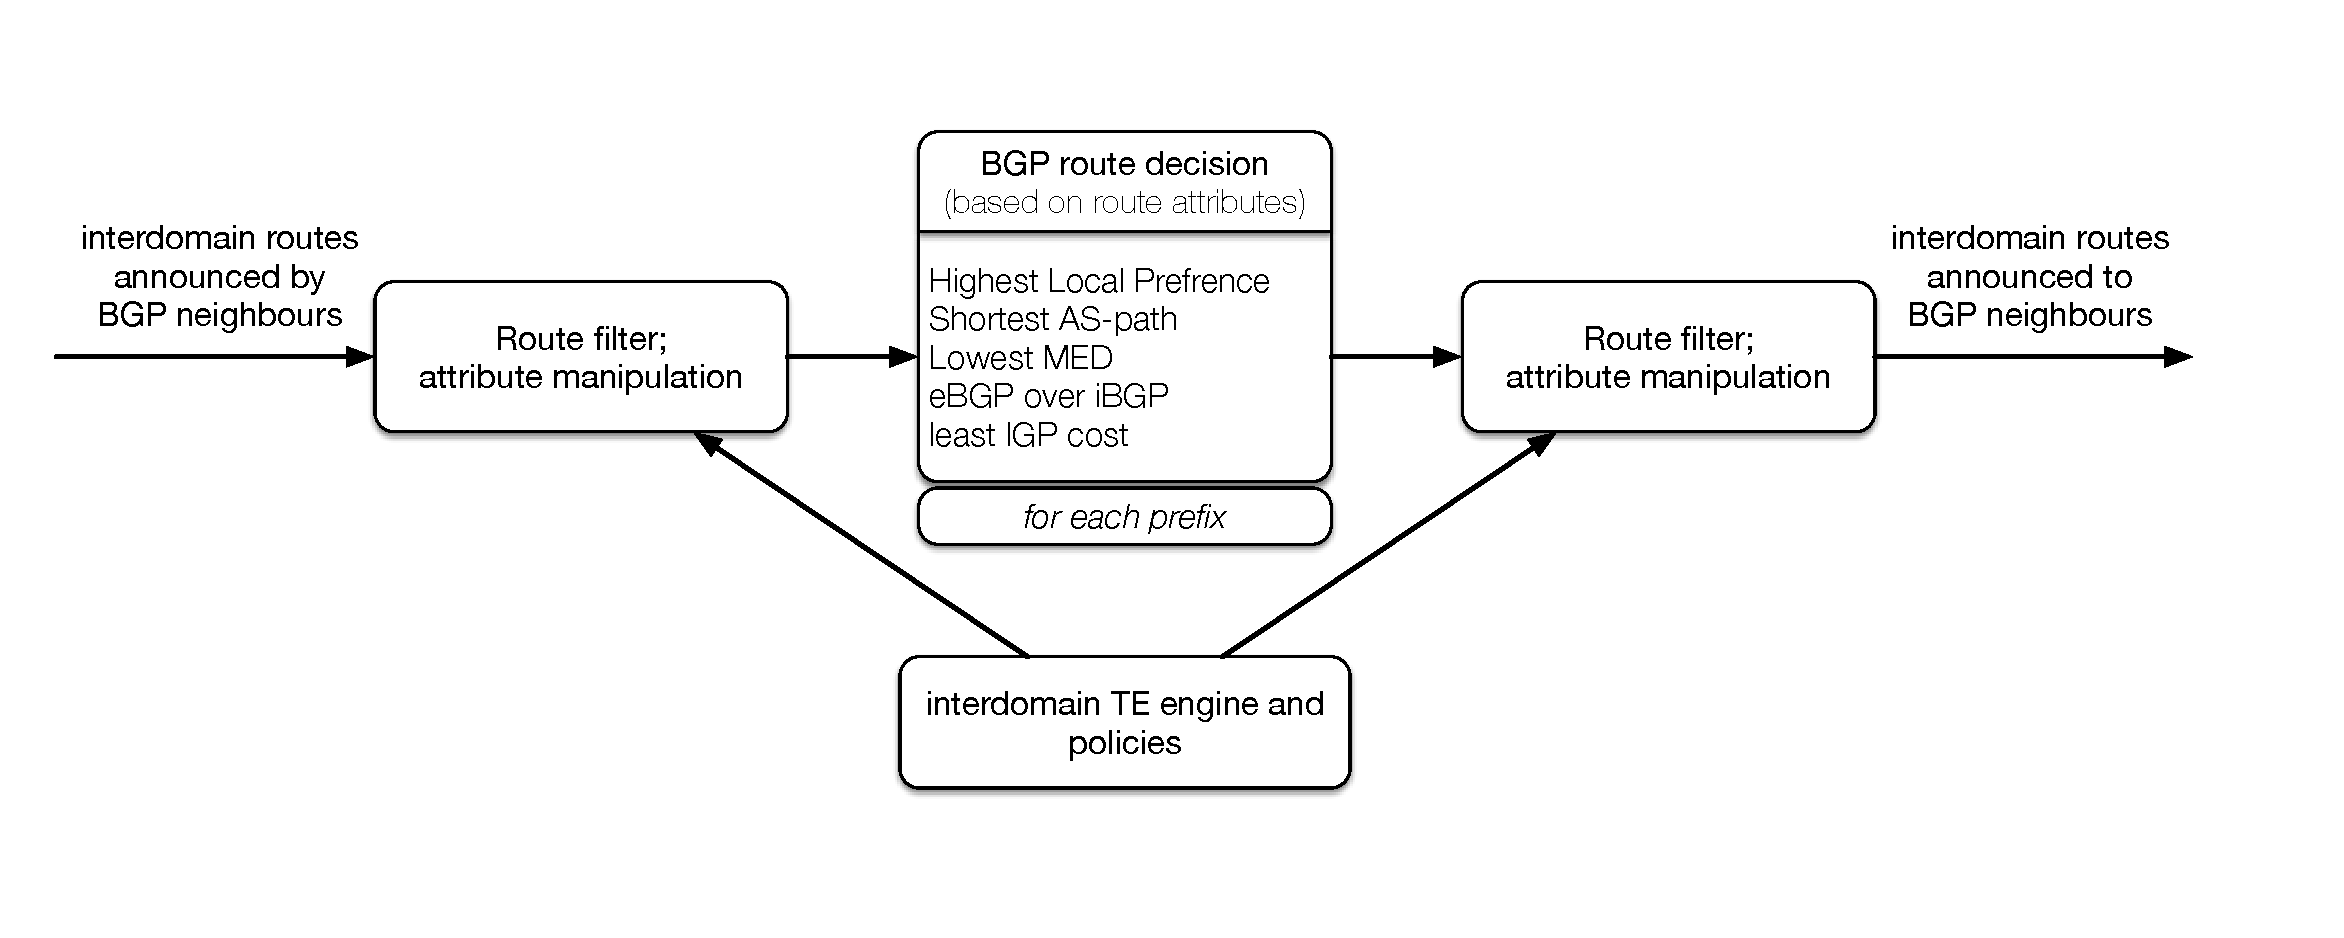
\includegraphics[width=1.3\textwidth]{gfx/chap1/bgp_decision.pdf}
\caption{Work flow of \acf{BGP} route selection and propagation within an \acf{AS} and the interaction with interdomain \acf{TE}.}
\label{fig:bgp_decision}
\end{figure}

Interconnection of tens of thousands of independently manged networks known as \acf{AS} forms Internet.
Routing that happens among those ASes is referred to as 
\textit{interdomain routing}.
In order to exchange interdomain routes, each AS uses \acf{BGP}~\cite{bgp4}, a path vector routing protocol, to communicate with other ASes.
Each AS announces its own routes (routes towards its own prefixes) along with other routes learnt to its BGP neighbors as illustrated in Fig.~\ref{fig:bgp_decision}.
For each prefix, one single best route is selected by the BGP route decision route based on the BGP attributes attached to each route.
Each route can be filtered based on its attributes or altered before BGP route decision and announcement to its neighbors according to \acf{TE} policies~\cite{Quoitin2003, Gao2001a}.

\begin{figure}[!htb]
\centering
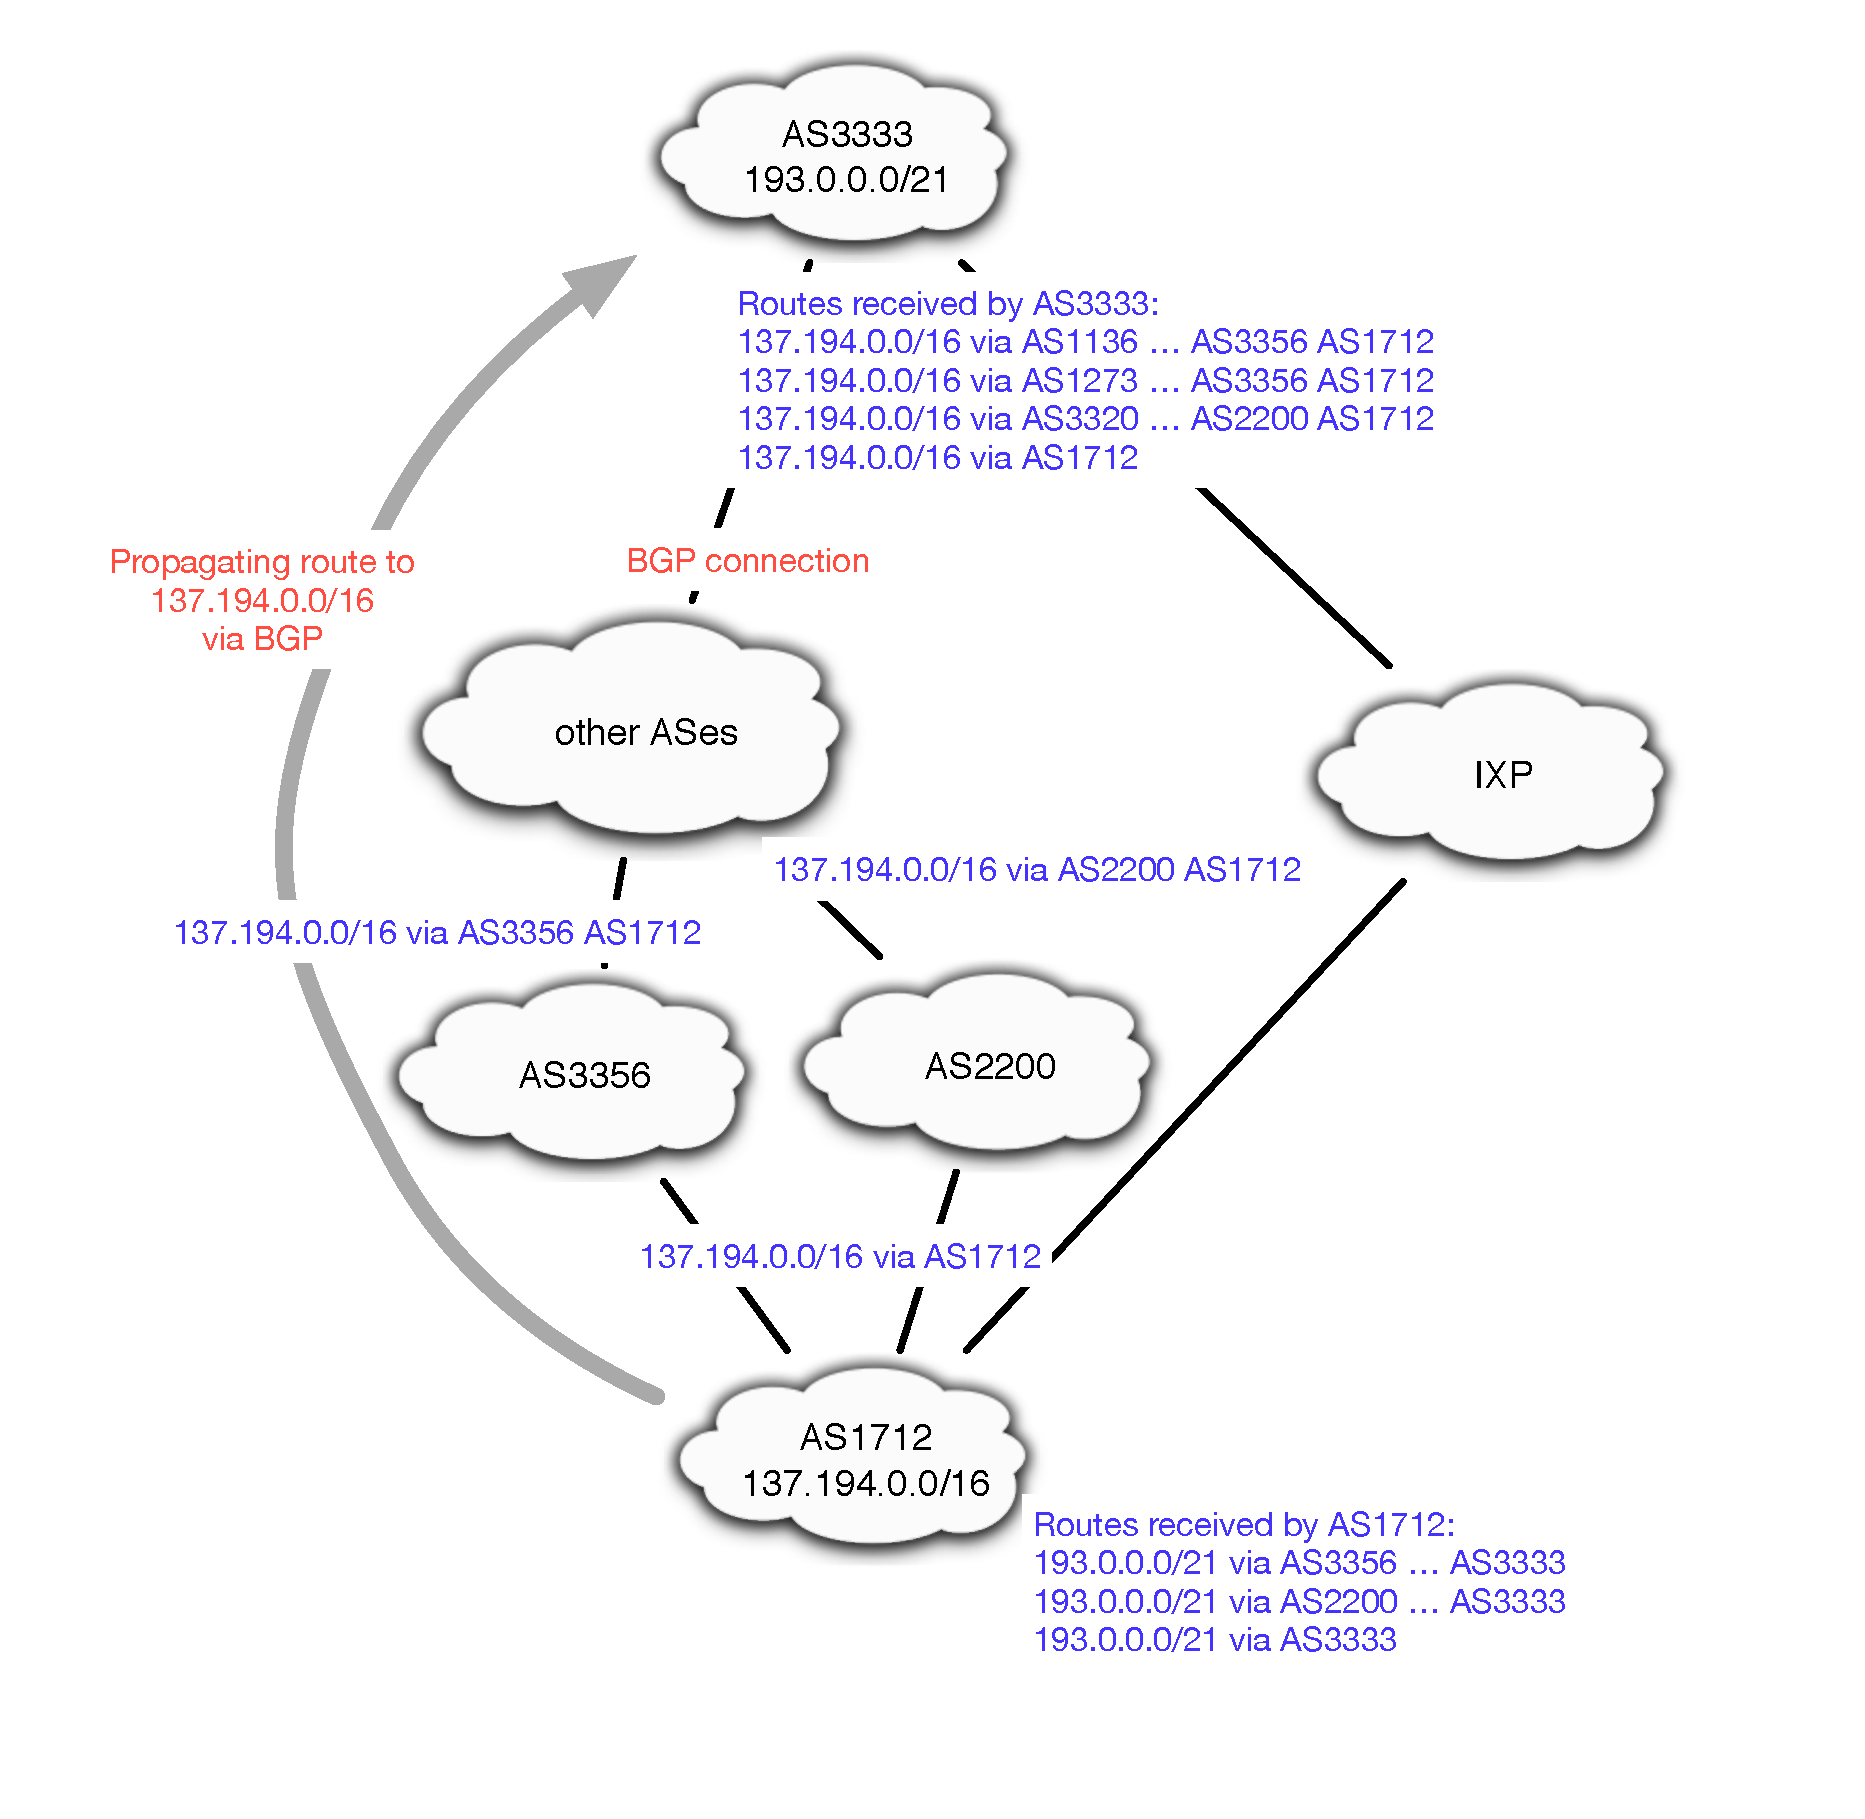
\includegraphics[width=1.1\textwidth]{gfx/chap1/bgp_route_propagation.pdf}
\caption{Interdomain route propagation via \ac{BGP}, an example of \texttt{137.194.0.0/16}. Networks illustrated are fictional.}
\label{fig:bgp_propa}
\end{figure}

Fig.~\ref{fig:bgp_propa} illustrates the propagation of interdomain routes to prefix \texttt{137.194.0.0/16} of AS1712 via BGP exchanges. Each AS inserts its own AS number when announcing the learnt route to other ASes, thus forming an AS path at the receiver side. When AS3333 learns the routes to \texttt{137.194.0.0/16} as depicted and AS1712 learns those to \texttt{193.0.0.0/21} in a similar way, the two ASes can exchange traffic across Internet using addresses within these two prefixes.

There are two types of ASes in above BGP exchanges: \textit{transit provider} and \textit{stub AS}.
Transit provider refers to ASes that offer to route traffic not originated from nor sent to itself, as a commercial service.
For that purpose, a transit provider announces to its clients all the interdomain routes its learns and to its other BGP neighbors the routes to its clients.
In Fig.~\ref{fig:bgp_propa}, AS3356 and AS2200 are transit providers of AS1712. They help announce the route to prefix \texttt{137.194.0.0/16}
to the rest of Internet.
On the contrary, a stub AS only cares about sending out its own traffic and becoming reachable to others.
Accordingly, it only announces to its transit providers its own routes. AS1712 is a stub AS in Fig.~\ref{fig:bgp_propa}, as it does not relay interdomain routes for other ASes, e.g. AS1712 will not announce to AS3356 the route to \texttt{193.0.0.0/21} learnt from AS2200. Consequently no traffic toward ASes other than itself shall arrive at it.

Besides the transit relationship described above, peering is another type of route and traffic exchange that can happen between two ASes under BGP. Two ASes in peering relationship exchange with each other their own routes, so that they can directly communicate without employing a transit provider.
In Fig.~\ref{fig:bgp_propa}, AS1712 and AS3333 directly peer at an \ac{IXP}.
\ac{IXP} is a collocation facility that eases establishment of peering relationship, thus is transparent to BGP route exchanges.

\section{Interdomain TE}
Thanks to transit and peering relationship, AS3333 and AS1712 in Fig.~\ref{fig:bgp_propa} may receive multiple routes to a certain destination prefix. Meanwhile, they can as well potentially receive traffic from multiple neighbors.
Such diversity in route brings up two questions: 1) which routes are the best; 2) how to route corresponding traffic on the desired paths.
The efforts spared in answering these two questions are referred to as \textit{interdomain \ac{TE}}~\cite{Quoitin2004a,Quoitin2003,Feamster2003}.

The first question deals with the objective of \ac{TE}. In general, one aims at optimizing the cost and/or performance of transmission.
The second question explores the method traffic steering.
We summarize the current practices, their limitations and challenges for incoming and outgoing traffic separately in this section.

\subsection{Outbound interdomain TE}
How to select the best route for each destination prefix and send out the traffic correspondingly is known as outbound TE. 
An AS has the total control over the egress routes to be employed in reaching each destination prefix. Common practice is to tune \textit{local preference} BGP attributes~\cite{Wang2008} before BGP route decision as illustrated in Fig.~\ref{fig:bgp_decision}. 
Therefor the challenge is rather on the composition of best routes in terms of cost and performance.

The cost of interdomain transmission depends on the the amount of traffic exchanged on links purchased from transit providers~\cite{drpeering-95th}.
Meanwhile, whether these transit links are congested impacts as well the transmission performance.
Hence, outbound TE resolves in routing an appropriate amount of traffic on each available transit links to lower the transit cost while not surpassing the capacity of each link (especially the cheapest one).

\citet{Goldenberg2004} formulated this quest as a minimum-cost multi-commodity flow problem when avoiding transit link congestion under transit cost constraints.
\citet{Uhlig2004b} fulfills the same goal while minimizing the number of route changes required with the help of traffic volume prediction.
\citet{Zhu2014} avoids congestion on transit links by including border router queue length in route decision.

Indeed, it is unwise to greedily saturate the cheapest transit link while residual capacity is available through other transit providers.
However, there are many other factors that may as well put transmission performance in danger.
The minimum delay of Internet transmission is dominated by the physical length traversed by a route. 
On top of that, transient events like congestion can as well happen in the middle of Internet~\cite{Akella2003, Luckie2014}, independent of traffic load on transient links.
In order to first learn the presence of these issues and then optimize the routing against these events, end-to-end performance measurement is indispensable in cumulatively reflecting the contribution from each element on the forwarding chain, including the transit links.


\subsection{Inbound interdomain TE}
Inbound TE takes care of the incoming traffic distribution on available links connecting to other ASes.
Through Fig.~\ref{fig:bgp_decision} and \ref{fig:bgp_propa}, we learn that the paths that incoming traffic takes is decided by distant senders, e.g. AS3333 decides which one to use to reach \texttt{137.194.0.0/16} of AS1712.
What AS1712 can do to influence the the route decision of AS3333 is by 
filtering route or tuning certain BGP attributes when announcing its own route to its BGP neighbors.
Some common practices are: selective announcement, more specific announcement, AS path prepending, setting \ac{MED}~\cite{Wang2008}.

These approaches are not perfect. Selective announcement introduces reachability risks, while more specific announcement gives rise to \ac{RIB} inflation. AS path prepending is as well shown to be not effective in avoiding using a specific transit provider~\cite{Quoitin2004a}. BGP community~\cite{Donnet2008, Shao2015} and later on redistributed communities~\cite{Quoitin2002} allow finer grained operations with better certainty. However, it requires the support from transit providers. 

The above researches suggest that it is very difficult if not totally impossible for an AS to have a fine control over the paths employed by incoming traffic. In this context, defining the best paths in terms of cost of performance is meaningless without effective method enforcing them. 

Therefore, the focus of other researches are rather on traffic steering methods.
Incoming path can be dictated by changing the traffic source address through encapsulation~\cite{Liu2008} or \ac{NAT}~\cite{Sun2015}. However, traffic with source addresses outside the prefixes announced to its BGP neighbors can be dropped for security considerations~\cite{filtering}.
\ac{LISP} pushes such approach to a revolutionary level by introducing a separate addressing space in the core of Internet that enables plenty TE operations impossible with mere BGP~\cite{lisp}. Studies show fine-grained and dynamic inbound optimization is henceforth feasible with the deployment of \ac{LISP}~\cite{Iannone2007, saucez2011mechanisms, quoitin2007evaluating}.

\subsection{Software Defined Networking and interdomain TE}
Recently, \acf{SDN} contributes as well to interdomain TE. One outstanding idea is to delegate the TE tasks of an AS to a third party, where route decision and traffic steering are performed in a centralized manner in accordance to \ac{SDN} design philosophy. It is advocated that the interdomain TE can hence be done in a more cooperative way as conflicts of interest from multiple ASes can be solved centrally to obtain a larger optmality.
\citet{Kotronis2012} advances that such AS clusters under same TE service provider can be formed in an gradual way and eventually drives the evolution of the interdomain routing.
\citet{Gupta2014} focuses on the application of \ac{SDN} in a more specific network environment, \ac{IXP}, where members by nature forms a cluster of ASes that exchange their routing information along with their TE polices within one centrally managed facility. Application specific peering, e.g. only peer for the exchange of video traffic, is made possible under this framework.

\section{Scope of this thesis}
We stage the works of this thesis under BGP, while fully realizing \ac{LISP}, \ac{SDN} and etc. are promising directions to pursuit.
It is because BGP is still going to be the \textit{de facto} routing protocol of Internet in the foreseeable future, for the deployment of new routing mechanism must be incremental.
Till then,  BGP is what a majority of ASes has to live with. 
There are thus immediate needs for improvements.

We focus on outbound TE in this thesis, as inbound TE has been shown previously to be inherently difficult with BGP due to lack of effective traffic steering methods.

We target stub ASes (potentially multi-homed).
It is because \ac{CP}, \ac{HP} and \ac{ISP}, being major network types among stub ASes, are those who needs most outbound TE.
Moreover, dynamic route re-selection in those networks will not cast Internet-wide BGP route convergence issues, since they do not announce to other ASes any of other routes nor the updates.

Finally, we assume improving transmission performance is nowadays the major motivation for outbound TE in stub ASes.
Continuously decreasing transit price~\cite{transitprice, drpeering} and high \ac{IXP} growth rate worldwide~\cite{pchixp} indicate that routing traffic throughout Internet now faces less monetary constraints but rather encounters a performance challenge that could be potentially lifted with geographical and topological connection diversity~\cite{Chiu2015}.


\section{Measurement-based TE and motivations}

BGP itself is one big obstacle in the pursuit for better transmission performance.
As shown in Fig.~\ref{fig:bgp_decision}, its route decision mechanism is unaware of the performance characteristics of candidate paths~\cite{Yannuzzi2005}.
Yet, not all interdomain routes offer the same transmission performance. \citet{Akella2003} pointed out that bandwidth bottleneck can be within certain \acp{ISP} or on the links between \acp{ISP}, suggesting that the choice of transit provide is not without impact on transmission performance.
Further, \citet{Akella2003a} reported a $30\%$ potential performance gain involving dynamic route re-selection that an AS could achieve with multi-homing.
%\cite{Akella2004} advocates that this gain is not far away from that of overlay networking.

In order to actually realize this performance gain, a system that dynamically selects for each destination the best performing route according to real-time measurements is required, i.e. \textit{measurement-based TE}.
\citet{Akella2008} presented a demo implementation of such a system that makes outbound TE decision based on end-to-end delay measurements. Only 100 destinations are emulated in this work, far less than the actually number a stub AS might face on a daily base. Best route is chosen based on the \ac{EWMA} of past \acf{RTT} measurements. The work shows that the best overall transmission performance is achieved when route decision is made upon last single measurement. However, considering the noisy nature of \ac{RTT} measurements, such a simplistic approach can lead to overwhelmingly frequent path changes that is not necessary. Moreover, treating Internet as a blackbox for delay measurements does not provide useful and necessary visibility regarding the actual network events that cause significant performance degradation and hence falls short in justifying the TE decisions made. 

In order to address these concerns and narrow the gap between the concept of measurement-based TE and a working system~\cite{b6}, we 
study in this thesis traffic volume, delay and path measurements to improve the scalability, measurement interpretation and performance visibility of such a system.


\section{Roadmap}
\subsection{Building blocks of measurement-based TE}

\begin{figure}[!htb]
\centering
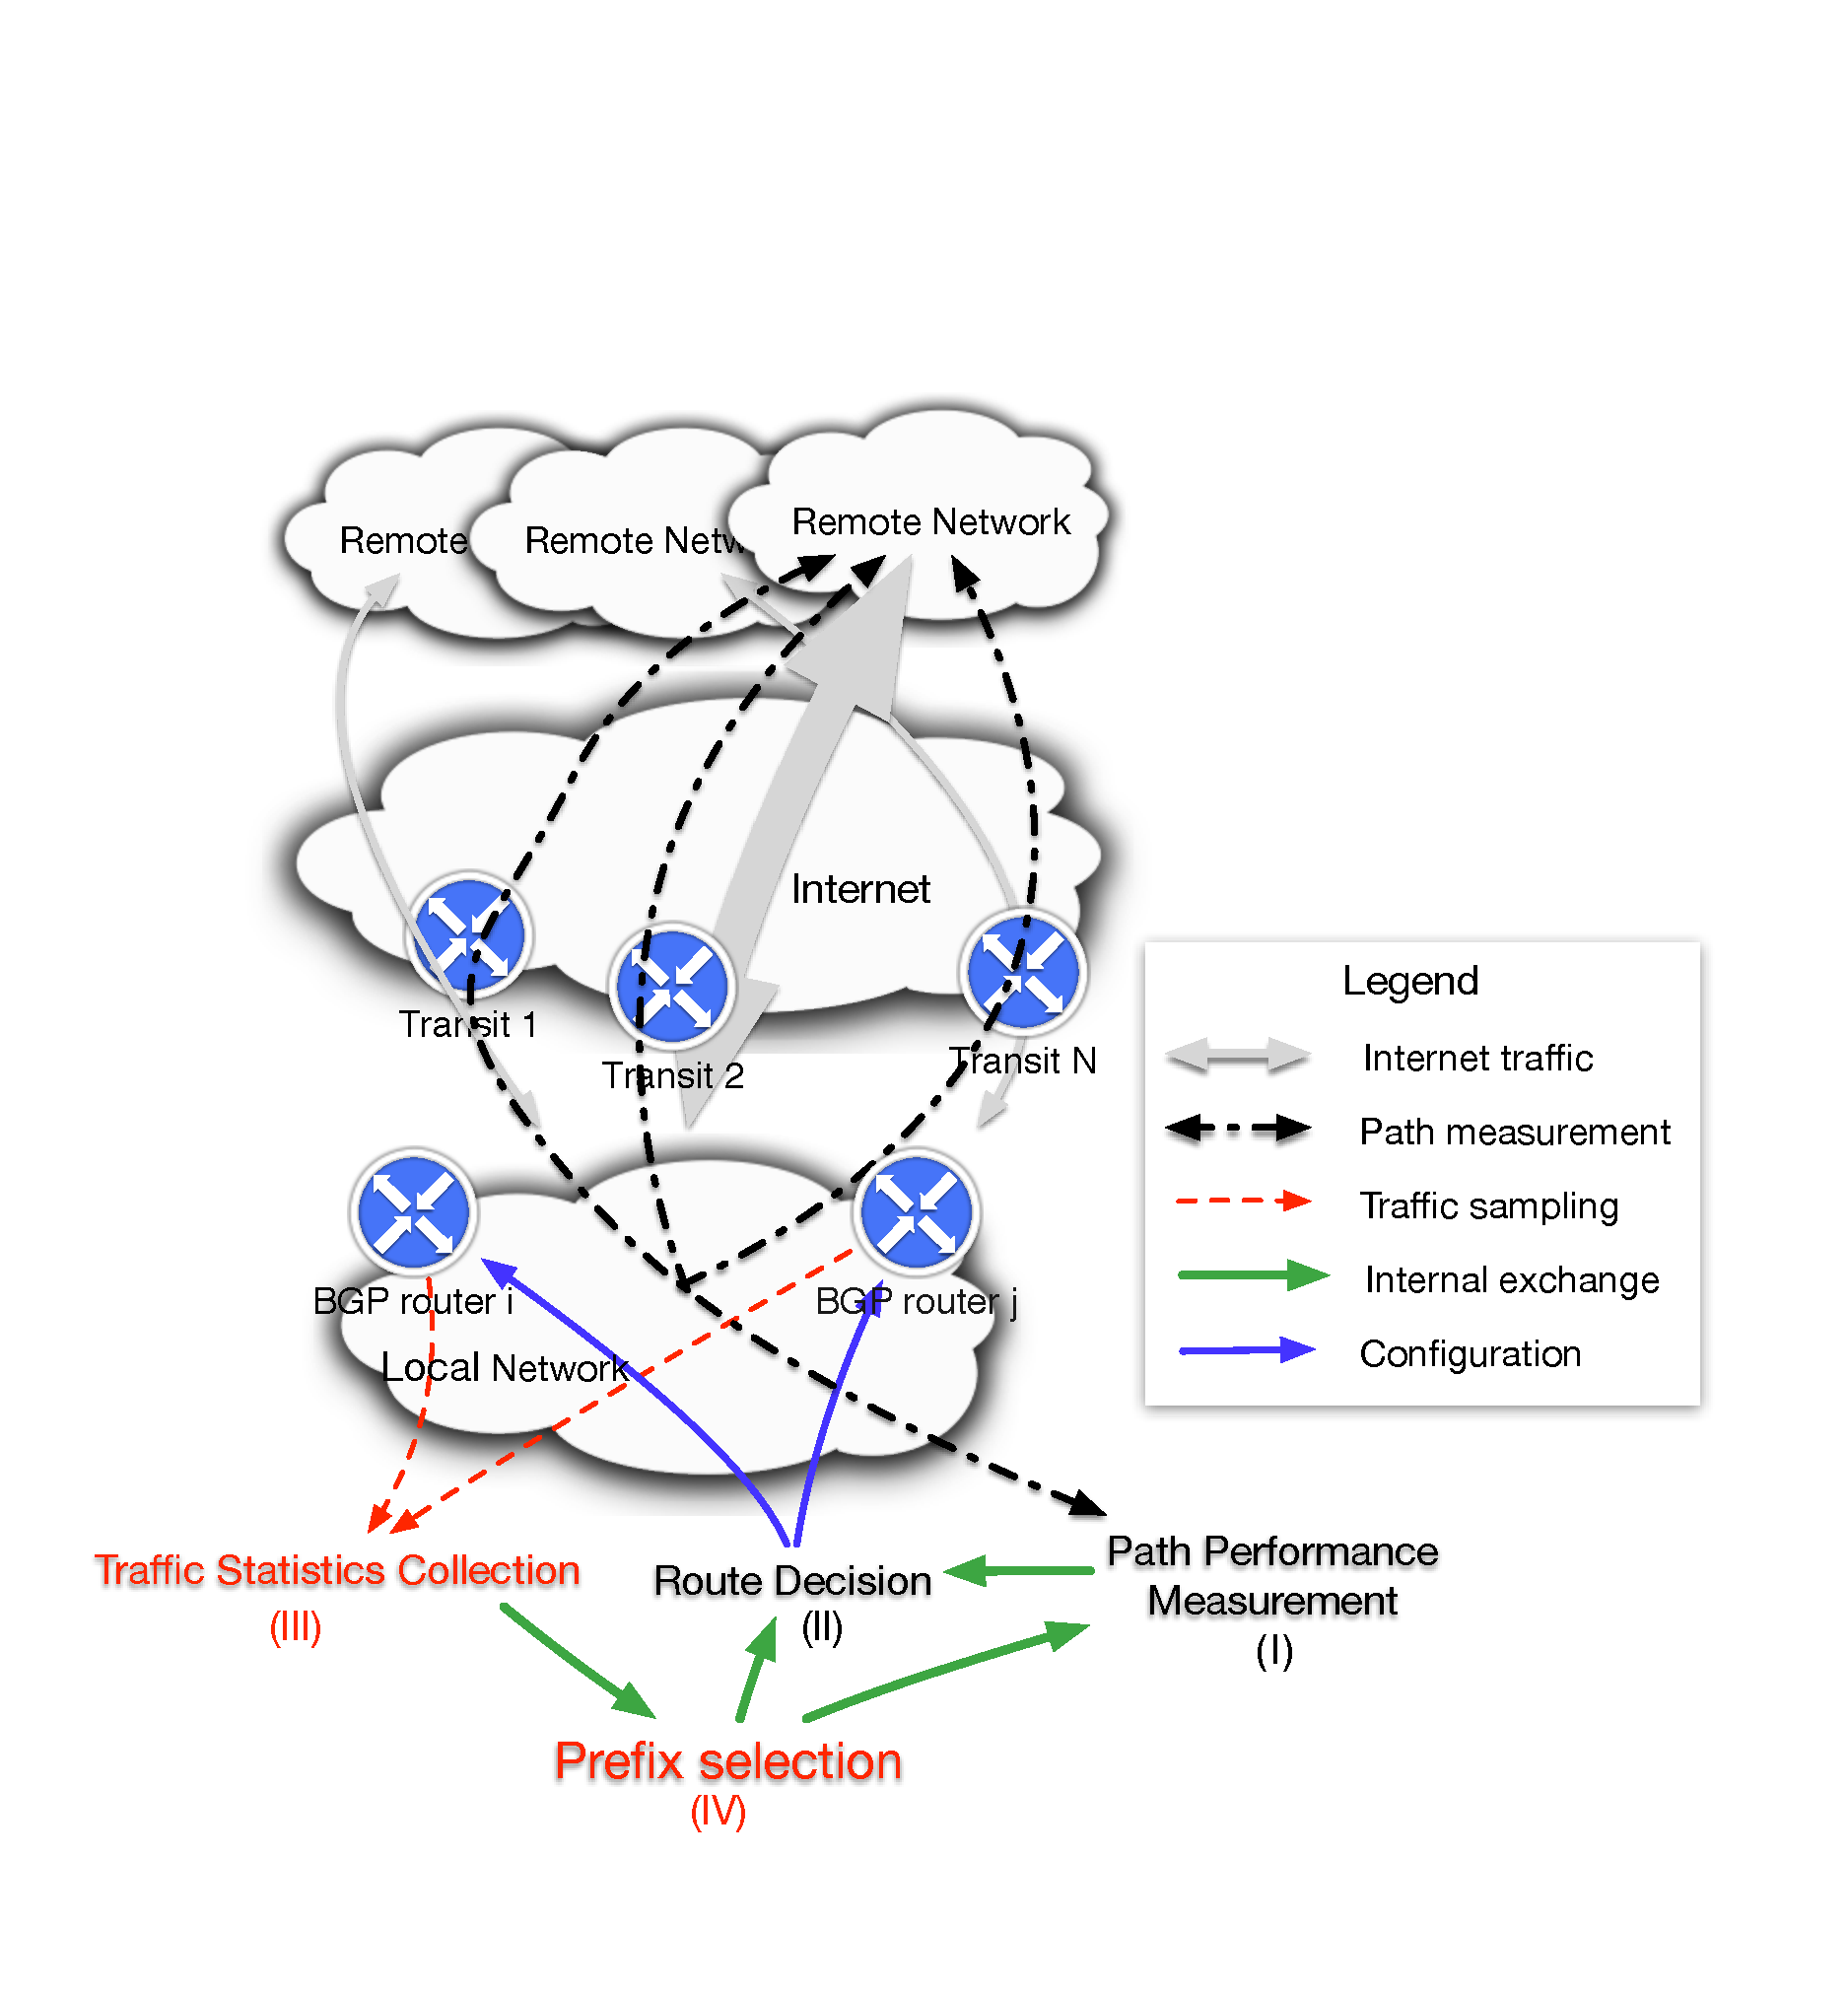
\includegraphics[width=\textwidth]{gfx/chap1/archi.pdf}
\caption{Building blocks of measurement-based inter-domain TE system.}
\label{fig:archi}
\end{figure}

A measurement-based interdomain TE platform has two essential building blocks illustrated in black in Fig.~\ref{fig:archi}: (i) path performance measurement and (ii) route decision.
Since each destination prefix may have multiple available routes, the platform has to measure in a repeated manner the end-to-end performance, more specifically \acf{RTT}, over all these routes. 
For each destination prefix, a couple of hosts with known open ports, e.g. 80, 443, are discovered and used as probing destination in delay measurements.
Once fed with performance metrics, route decision engine dictates for each destination which is the best route at a each moment and imposes it on BGP border routers.

\subsection{Prefix selection: focus on most important destinations}
However, a scalability issue presents in the above design as a stub AS can exchange with up to around 100k destination prefixes.
Continuous performance monitoring to all these destinations over all available paths is going to be prohibitively costly.
\citet{Feamster2003} already realize this issue and propose to focus on popular destinations.
However, no solution is given.
In Chapter~\ref{sec:pref_selec} we tackle the selection of prefixes associated with important traffic volume by studying their temporal dynamism at different time resolutions. Two additional building blocks (in red) are hence added to Fig.~\ref{fig:archi}.

\subsection{RTT measurements with RIPE Atlas}
Studies in Chapter~\ref{sec:pref_selec} solely base on the measurement data collected by a proprietary TE platform~\cite{b6} from client networks. Such working trace from real networks increases the credibility of our observation. However, it brings as well reproducibility concerns.
In Chapter~\ref{sec:ripe_atlas}, we first justify our choice of using RIPE Atlas~\cite{atlas} as our source of path and delay measurements for later researches.
We then discuss a data quality issue originated from the measurement platform.

With the openly accessible measurements from RIPE Atlas, we investigated another data quality issue, which is specific to interdomain TE this time. We employ unsupervised learning methods to reveal the inherent structure of a group of delay measurements on a same AS path.

During the above study, we notice an interesting case where several RTT time series exclusively share a similar shape at about the same moment.
We thus find it promising to infer the actually location of shared RTT changes by grouping RTT time series of similar shapes. To that end, we study the application of time series clustering methods to RTT measurements and discuss their limitations.

\subsection{Change detection for RTT measurements}
The case of RTT time series with similar shapes leads to further studies in Chapter~\ref{sec:cpt_rtt} and \ref{sec:infer}. Chapter~\ref{sec:cpt_rtt} studies the application of changepoint detection methods on RTT measurements. These methods detecting significant changes in time series is regarded as an expressive way to simplify the representation of RTT measurements. Meantime, we realize that the detected moments of change can serve as an informative and robust trigger for route re-selection.

To quantify the change detection performance on RTT measurements, we build an evaluation framework and benchmark several candidate methods.
The temporal correlation between RTT changes and routing events are as well studied and illustrated.

\subsection{Inferring the location of RTT changes}
With simplified data representation enabled by changepoint detection, we study the method inferring the location of detected RTT changes in Chapter~\ref{sec:infer}.
Knowing the location of RTT changes are of significance in measurement-based interdomain TE, especially for a non-negligible part of destinations that we are not able to measure directly. It provides visibility to avoid certain problematic paths when end-to-end measurements are absent.

For that purpose, we first group RTT time series undergoing same RTT changes with the help of changepoint analysis.
Then inference logic are developed to attribute RTT change to ASes and links basing on two simple and intuitive assumptions.
Visualization tools are developed to illustrate the inference process and the inferred location of change on an AS-level topology learnt from path measurements.
